\chapter{Code contribution}
\section{WolfSSL}
\label{app:modifs}

The table below is a \texttt{git diff} between our wolfSSL repository and the official one. It gives an idea about the work done to implement our MPDTLS extension. This can be reproduced dynamically on our Github repository page \cite{wolfssl-mpdtls}.

\textsf{
\begin{center}
\begin{tabularx}{.9\linewidth}{Xr}
.gitignore                      & \textcolor{gitgreen}{+1} \textcolor{gitred}{-1}      \grule\rrule\garule\garule\garule \\
\hline
README                          & \textcolor{gitgreen}{+7} \textcolor{gitred}{-0}      \grule\grule\grule\grule\grule\\
\hline
README.md                       & \textcolor{gitgreen}{+6} \textcolor{gitred}{-0}      \grule\grule\grule\grule\grule\\
\hline
configure.ac                    & \textcolor{gitgreen}{+36} \textcolor{gitred}{-0}     \grule\grule\grule\grule\grule\\
\hline
src/internal.c                  & \textcolor{gitgreen}{+1,844} \textcolor{gitred}{-65} \grule\grule\grule\grule\garule\\
\hline
src/io.c                        & \textcolor{gitgreen}{+77} \textcolor{gitred}{-3}     \grule\grule\grule\grule\garule\\
\hline
src/ssl.c                       & \textcolor{gitgreen}{+358} \textcolor{gitred}{-3}    \grule\grule\grule\grule\garule\\
\hline
src/tls.c                       & \textcolor{gitgreen}{+187} \textcolor{gitred}{-2}    \grule\grule\grule\grule\garule\\
\hline
wolfssl/error-ssl.h             & \textcolor{gitgreen}{+5} \textcolor{gitred}{-2}      \grule\grule\grule\rrule\garule\\
\hline
wolfssl/internal.h              & \textcolor{gitgreen}{+253} \textcolor{gitred}{-4}    \grule\grule\grule\grule\garule\\
\hline
wolfssl/ssl.h                   & \textcolor{gitgreen}{+59} \textcolor{gitred}{-1}     \grule\grule\grule\grule\garule\\
\hline
wolfssl/wolfcrypt/error-crypt.h & \textcolor{gitgreen}{+5} \textcolor{gitred}{-0}      \grule\grule\grule\grule\grule\\
\hline
wolfssl/wolfcrypt/types.h       & \textcolor{gitgreen}{+3} \textcolor{gitred}{-1}      \grule\grule\grule\rrule\garule
\end{tabularx}
\end{center}
}

The largest part of our work is concentrated inside the \texttt{internal.c} file. This is really the core of the library since it treats every messages. It is in this file that all the \textit{Do}Functions and the \textit{Send}Functions described in Chapter \ref{chap:implementation} are implemented. All the initialization and creation of the structures used to store information about the flow including feedback and heartbeat are also done there.

All the API calls are implemented inside \texttt{ssl.c} such as the \texttt{use\_multipath()} or the \texttt{add\_new\_addr} functions. They are checking the input data from the user and make the appropriate calls inside \texttt{internal.c}.

The heartbeat extension has required some modifications inside \texttt{tls.c} to be fully supported. This is also where we had to put our Hello extension for the extension discovery during the handshake.

The file \texttt{io.c} has slightly been modified to integrate our schedulers outside the core of the library and make it easily replaceable.

Some minor modifications have also be made in other files to support our new option \texttt{--enable-mpdtls} during the building process.



\section{Wireshark}
\label{app:wireshark}

In this section we present our contribution to Wireshark \cite{wireshark} in order to support our new messages. As you can see we have mainly modified the dtls dissector to detect our packets and indicate how to format them once they are decrypted.

\textsf{
\begin{center}
\begin{tabularx}{.9\linewidth}{Xr}
.gitignore                      & \textcolor{gitgreen}{+2} \textcolor{gitred}{-0}      \grule\grule\garule\garule\garule \\ \hline
epan/dissectors/packet-dtls.c & \textcolor{gitgreen}{+444} \textcolor{gitred}{-0}      \grule\grule\grule\grule\grule\\ \hline
epan/dissectors/packet-ssl-utils.c & \textcolor{gitgreen}{+11} \textcolor{gitred}{-0}      \grule\grule\grule\grule\grule\\ \hline
epan/dissectors/packet-ssl-utils.h & \textcolor{gitgreen}{+7} \textcolor{gitred}{-1}      \grule\grule\grule\grule\garule\\ \hline
epan/dissectors/packet-ssl.c & \textcolor{gitgreen}{+5} \textcolor{gitred}{-0}      \grule\grule\grule\grule\grule
\end{tabularx}
\end{center}
}

Figure \ref{fig:trace} is a typical MPDTLS communication we can observe with Wireshark. Note that all the new packets are correctly identified.

\begin{figure}[!ht]
\centering
\includegraphics[width=0.8\textwidth]{images/trace.eps}
\caption{Wireshark trace of MPDTLS traffic}
\label{fig:trace}
\end{figure}


An example of how a \texttt{CIM} packet is formatted with Wireshark is shown on Figure \ref{fig:cimdetail}. We can see all advertised addresses together with their port number. 

\begin{figure}[!ht]
\centering
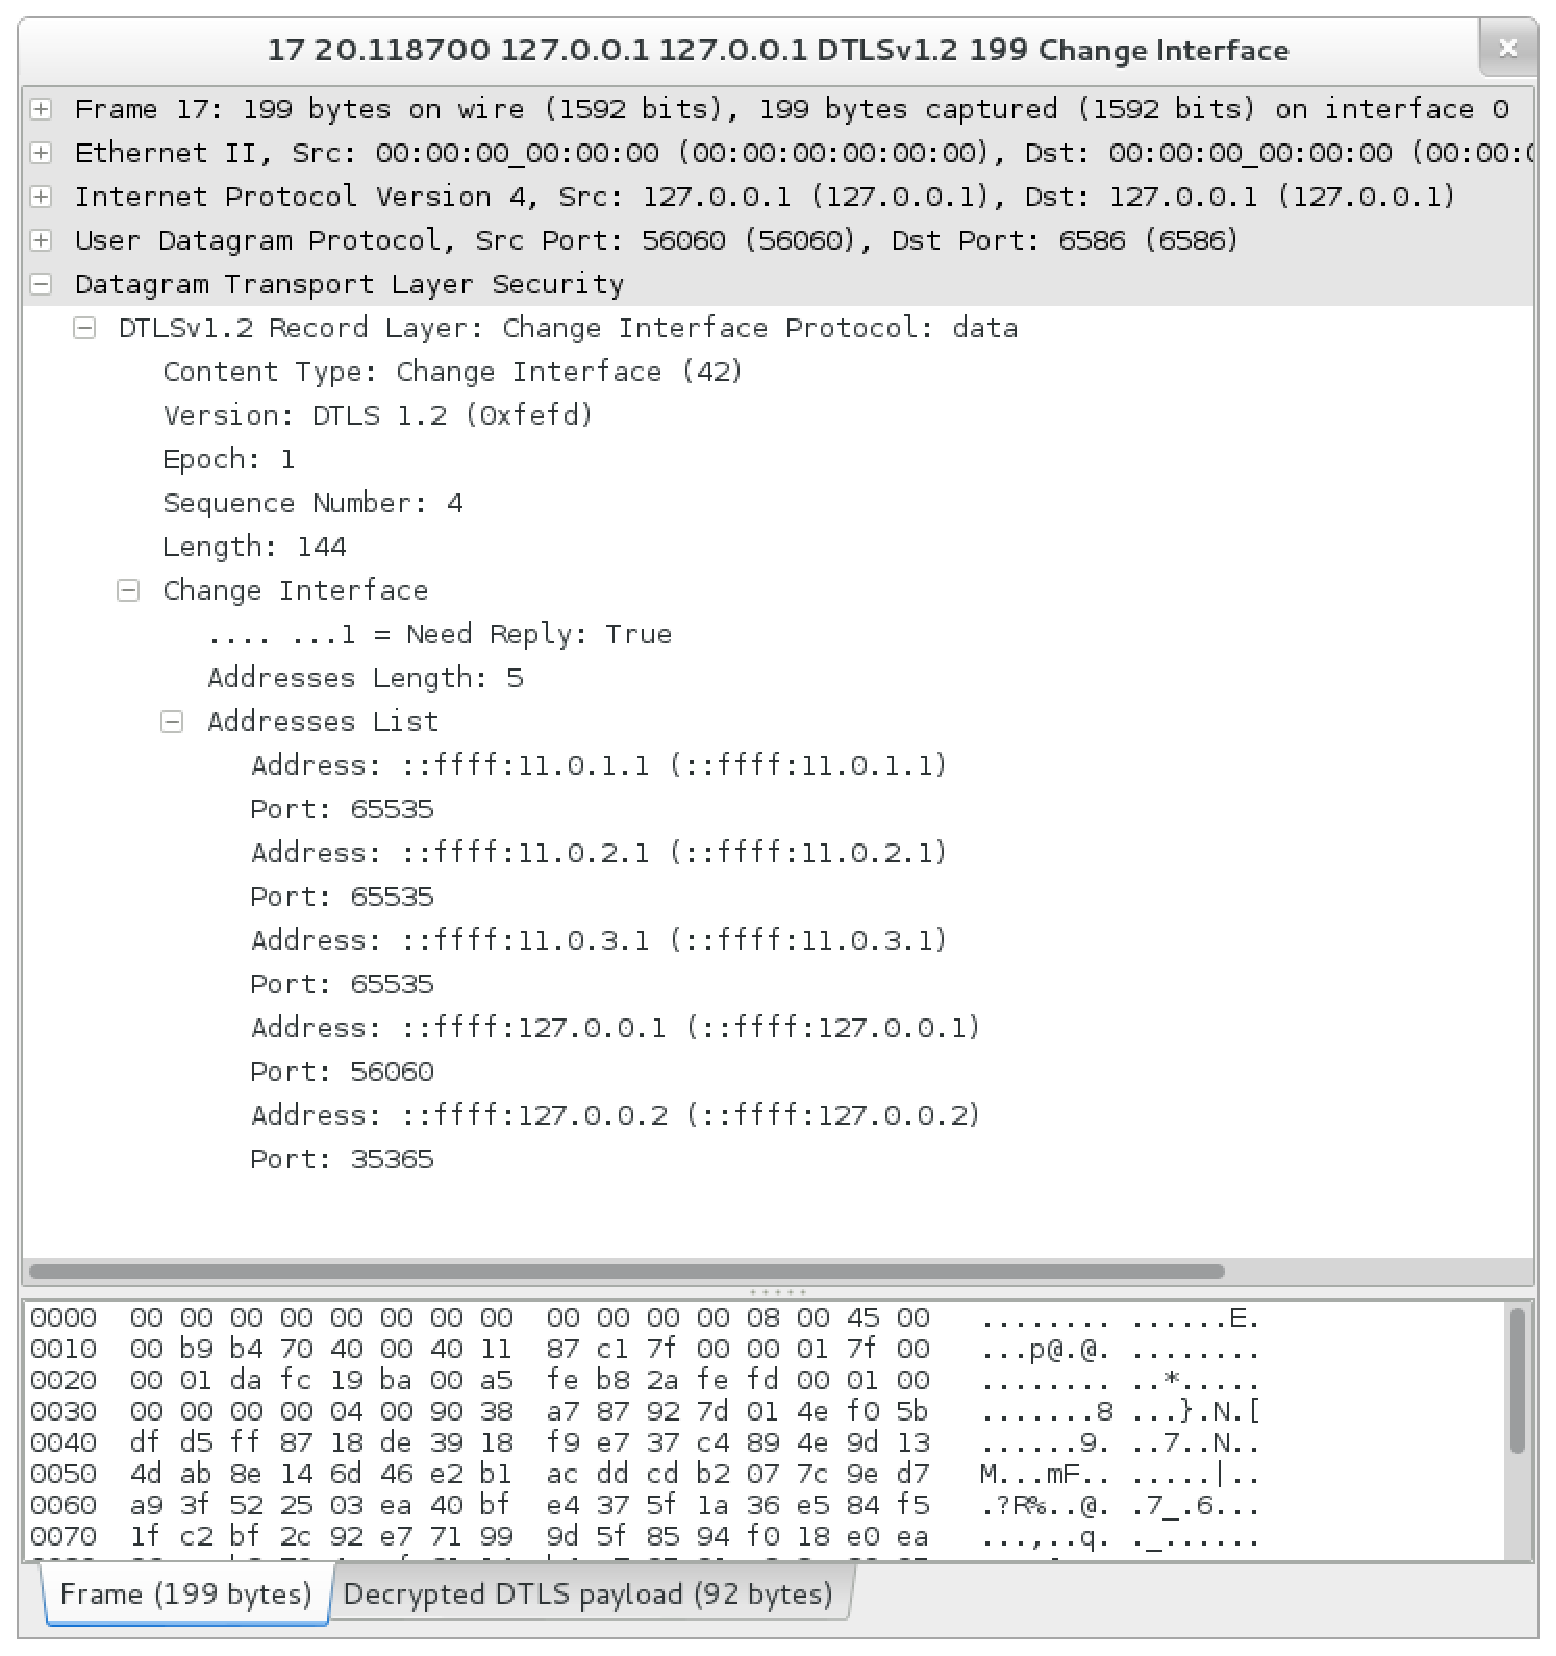
\includegraphics[width=\textwidth]{images/cimdetail.eps}
\caption{The decrypted content of a CIM with Wireshark}
\label{fig:cimdetail}
\end{figure}
